
\section{Elementary Particles}\index{EP}
One of the questions that we, as human beings, have been asking since we started thinking, is ``What is the universe made up of and what holds it together?'' A long time ago, Democritus tried to answer the first part by defining “atoms”, although his definition of the atom was quite different from what we know about the atom today. In the last couple of centuries, we have come a long way in terms of answering the questions about the composition of matter and the glue that holds it together and  gives us the form of the universe we see today.
The quest to answer the question ``What is matter made of?'' 
has been much like unraveling Russian nesting dolls (Figure ~\ref{fig:fig1}). 
Everything, such as chairs, tables, you, and me are 
made up of different kinds of molecules. Every molecule is made up of different kinds of atoms. All atoms, it turns out, even if they are different, have very similar structures; they all have one nucleus around which electrons revolve. The nucleus is made up of protons and neutrons. Protons are positively charged and electrons are negatively charged particles. The number of protons and electrons in a neutral atom are exactly equal so that the positive and negative charges cancel each other out.  All atoms are very similar in that they are all made up of protons, neutrons and electrons. However, a gold atom would be different from an iron atom or a hydrogen atom because they would have a different number of protons, neutrons and electrons.  




\begin{figure}[h]
\centering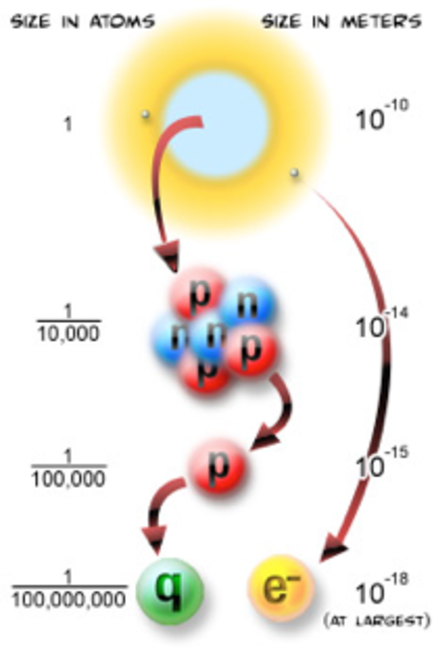
\includegraphics[scale=0.5]{./ElementaryParticles/Pictures/fi1.pdf}
\centering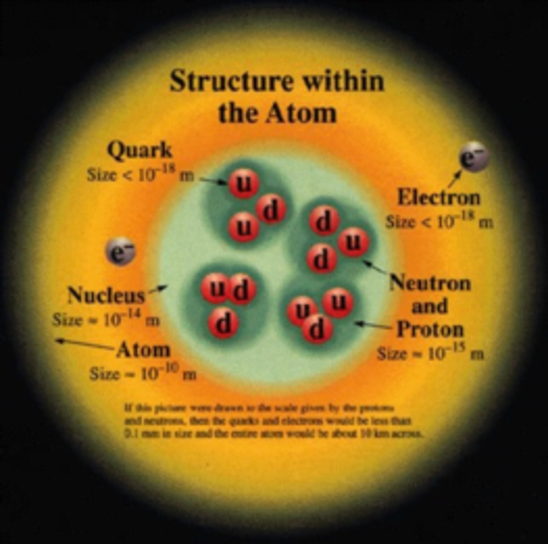
\includegraphics[scale=0.5]{./ElementaryParticles/Pictures/fig2.pdf}
\caption{The scale of fundamental particles}
\label{fig:fig1}
\end{figure}


However, the atom is not the last of our Russian dolls. We now know that every proton and neutron itself is made up of even smaller particles, called quarks. Electrons, on the other hand, appear to be fundamental particles; that is, they cannot be further decomposed. 
So, as of now, we can divide fundamental particles into two categories: Quarks and Leptons.  There are 6 types of quarks and 6 types of leptons. Quite symmetric, don't you think?  But the symmetry does not end here. They seem to form 3 pairs (we call them families or generations) as you can see from Figure ~\ref{fig:fig3}.

The three generations of quarks and leptons are very similar in that they have the same charge, spin etc. They differ in some internal quantum properties, but the most apparent difference is in the mass - – which increases as we go from 1st generation to 3rd. 
\\
As you can see from 
Figure \ref{fig:fig5} below, this difference is up to 5 orders of magnitude.


\begin{figure}[h]
\centering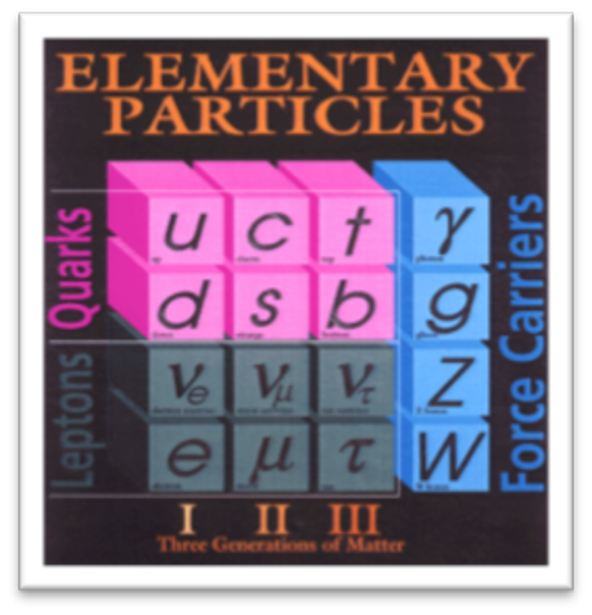
\includegraphics[scale=0.5]{./ElementaryParticles/Pictures/fig3.pdf}
\caption{Three generations of fundamental matter particles}
\label{fig:fig3}
\end{figure}


\begin{figure}[h]
\centering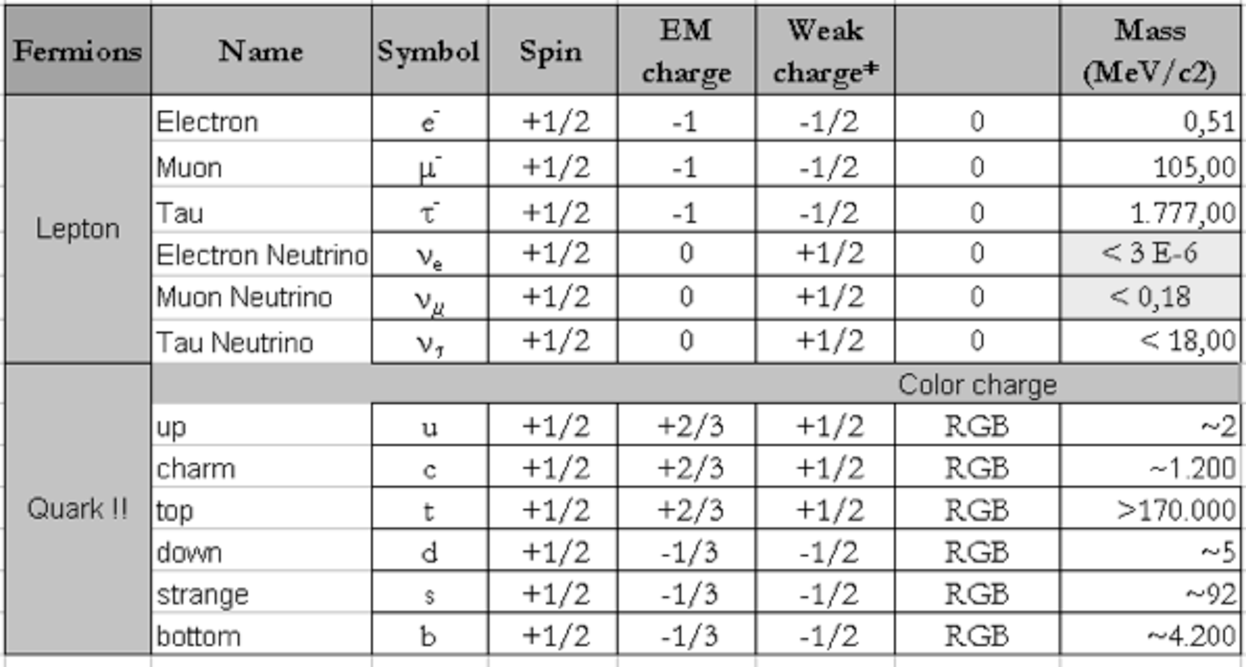
\includegraphics[scale=0.5]{./ElementaryParticles/Pictures/fig5.pdf}
\caption{Fundamental particles and their properties}
\label{fig:fig5}
\end{figure}


For every particle, there is also a corresponding anti-particle.  Usually they have simple names, such as an anti-up quark or anti-neutrino.  The anti-particle for the electron, however, has the special name, “positron”.  The existence of anti-matter was predicted when Paul Dirac unified quantum mechanics and Einstein's theory of special relativity.  The anti-electron was discovered a few years later (1932) by Anderson.

\section{Forces} 
There are a few other fundamental particles which do not make up matter directly, but instead are exchanged in interactions between matter particles. These force carrier particles, when exchanged between two matter particles, make these particles interact through the force which they are carriers of. 

There are four known fundamental forces
through which particles can interact and each has its own carrier particles.
 (see Figure ~\ref{fig:fig4}). 

1.	{\bf the strong nuclear force:} 
Only quarks can feel this force through the exchange of force carrier particles called gluons. This force is much stronger compared to electromagnetic force of repulsion between the same charge protons and keeps the atomic nucleus stable.


2.	{\bf the weak nuclear force:}
This is the force responsible for radioactive decay of atomic nuclei.  It has three force carrier particles, 
the $\rm{W^+}$, $\rm{W^-}$, and $\rm{Z^0}$ bosons. It allows one type of quark to turn into another, usually within the same generation.  
For example, a top quark can turn into a bottom quark by emitting a W boson.  It also allows a charged lepton to change into a neutrino. A muon can decay to a muon neutrino by emitting a W boson.  The weak force is also very important in the fusion reactions that power the sun.

3.	{\bf the electromagnetic force:}
The force between charged particles is mediated through the exchange of electromagnetic force carrier particles called photons.  This is the same photon that makes up the light that you see from the sun or a bulb. This is the force of attraction (repulsion) between opposite (same) electric charges or magnetic poles. 

4.	{\bf the gravitational force: }
The everyday force that keeps us safely on the surface of the earth and is felt by all particles with mass. The graviton, the theorized particle proposed to be the force carrier for gravity, 
has not been discovered yet. 


\begin{figure}[h]
\centering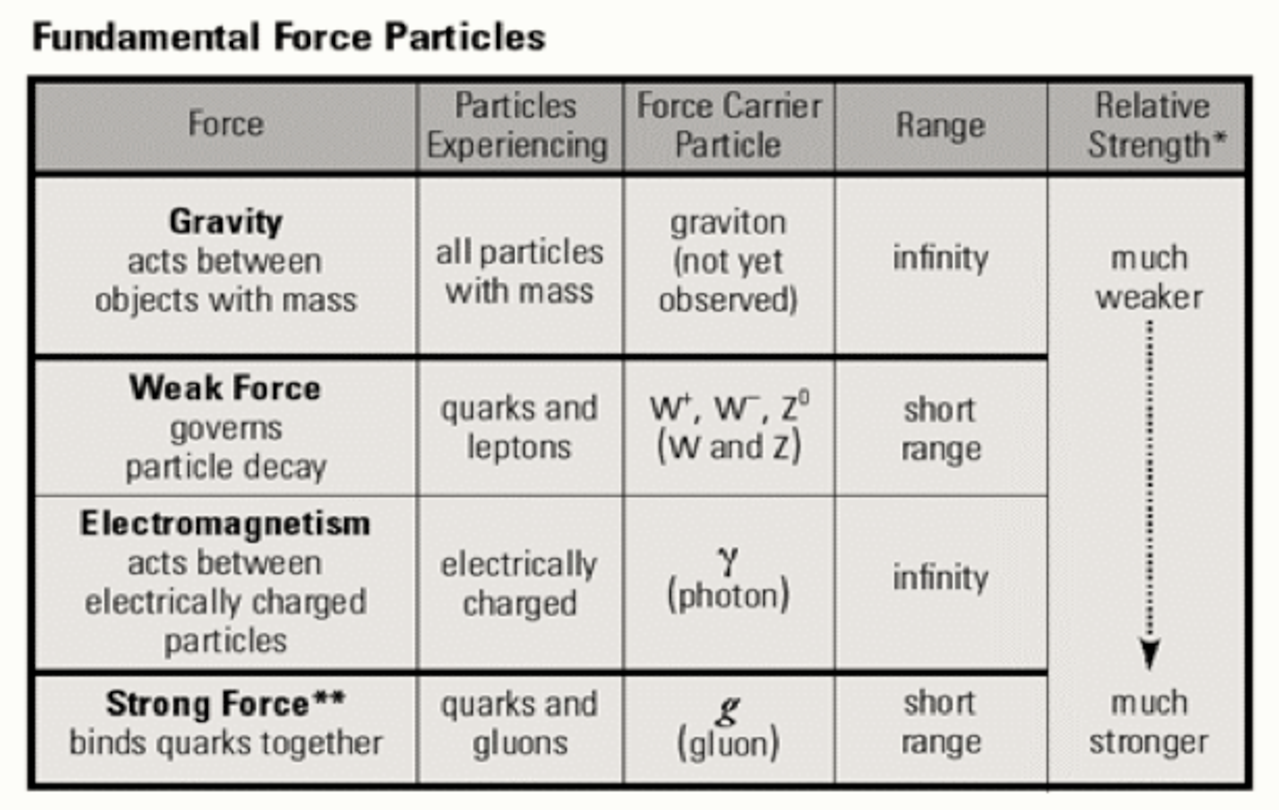
\includegraphics[scale=0.5]{./ElementaryParticles/Pictures/fig4.pdf}
\caption{Fundamental forces and corresonding force carrier particles}
\label{fig:fig4}
\end{figure}


\section{The world's shortest description of quantum mechanics}

One generally only attempts to learn about particle physics after studying quantum mechanics. Quantum mechanics is indeed fundamental to particle physics.  However, if a 
student's goal is to become involved in particle physics research, it is only strictly necessary to learn a small fraction of this fascinating subject.  In this section, we will try to describe the minimum amount of quantum mechanics you need to understand particle physics.  To really learn quantum mechanics, you need first to study differential equations, and most of you have not taken this yet.
Quantum mechanics is strongly related to one of the fundamental constants of nature, called 
$\hslash$ or h-bar.  $\hslash$ has the numeric value of ${\rm 1.054x10^{-34}}$ Js.  
If you see this constant in an equation, you know quantum mechanics is involved.
Often quantum mechanical systems involve quantization of energies.  The classic example is the energy states of the hydrogen atom (or any atom or molecule).  The electrons can only have certain energies.  These energies are associated with ``quantum numbers''.  The energies might be related to these numbers through a scale factor and a simple function of the numbers 
(although some of the quantum numbers are not related to energies but to other measurables).  The allowed values of energies are also often proportional to
${\rm \hslash}$

If an atom absorbs energy, it can only do this if the energy is the right amount to move the electron between one of these discrete states (approximately… there are corrections to this that are important only when being very precise).  Likewise, when an atom that is in one of the higher energy states “de-excites”, it can only emit photons with certain energies.

Energy quantization is an important property of  photons; the fundamental “packet” of electromagnetic radiation can only have energies that are integer multiples of the product of its angular frequency (${\rm \omega = 2 \pi f}$ where f is the frequency of the photon’s oscillation and ${\rm c = \lambda f}$  where c is the speed of light and ${\rm \lambda}$  is the photon’s wavelength) and ${\rm \hslash}$.  
Thus, ${\rm E=n \hslash \omega}$,  where n is an integer.

When you combine this with the energy levels of atoms, you get the characteristic absorption/emission spectra of atoms/molecules, which can be used to identify them (see Figure \ref{fig:light}).


\begin{figure}[h]
\centering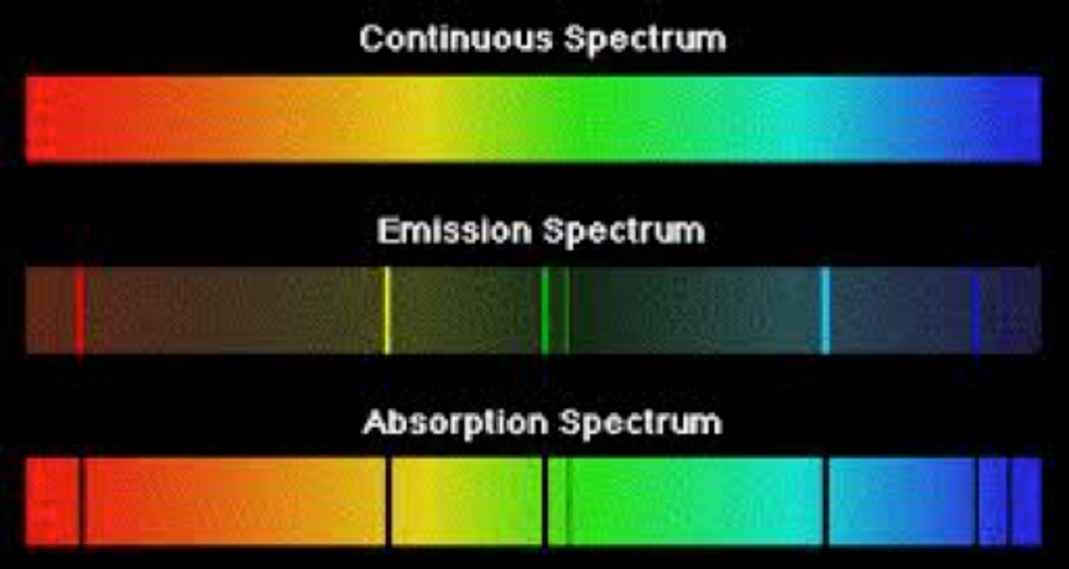
\includegraphics[scale=0.5]{./ElementaryParticles/Pictures/fig6.pdf}
\caption{absorption and emission lines}
\label{fig:light}
\end{figure}


Another important thing to know about quantum mechanics is that it is probabilistic in the sense that often for a given initial state (say, an electron aimed at a piece of metal) there may be many possible final states (say, amount of energy that the electron loses, and the deflection of the electron from its initial direction).  In quantum mechanics, you can only calculate the probabilities of the different possible outcomes; you cannot ever, even with perfect information about the initial state, predict exactly what the final state will be.

There is also the Heisenberg uncertainty principal.  The Heisenberg uncertaintly principal is a relation between two variables related by a Fourier Transform (google it if your curiousity is peaked).  The relationship says that if you precisely measure one of the variables, you can not have a precise measurement of the other.   Conjucate variables include energy with time and momentum with position.  What sets the scale for how well they can be measured?  Our friend ${\rm \hslash}$ of course.

Mathematically we can write:
\begin{equation}
\Delta E \Delta t \ge {\hslash \over 2}
\end{equation} 
where $\Delta$ is the accuracy in the measurement.

Also
\begin{equation}
\Delta p \Delta x \ge {\hslash \over 2}
\end{equation} 


 


\section{Standard model of particle physics}
Going back to the question, ``what is the universe made up of and what holds it together?'', 
our current understanding is that the matter in our visible universe is made up of quarks and leptons which interact with one another through force carrier particles.  There is a theory called ``the standard model of particle physics'' which describes this visible universe and, partly, the forces that hold it together. This theory, in principle, can describe all the physical process in chemistry and biology in terms of fundamental interactions. The standard model of particle physics describes phenomenon concerning three out of the four known 
fundamental forces: electromagnetic force, weak force and strong force. The formal name for the mathematical structure of this theory is “gauge-invariant quantum field theory”.  Gauge-invariant means that the properties of the bosons (force mediators) are determined by symmetries relating the matter fields (quarks and leptons). 
The fundamental particles and some of their basic properties are listed in 
Figure \ref{fig:fig4}.




\section{Properties of fundamental particles}
Every fundamental particle (for example an up quark) has exactly the same properties; no matter where or how it is produced. The quarks and leptons have similar properties like charge, mass, spin etc., but quarks have one extra property, called color. Just like particles with electromagnetic charge can only interact through the electromagnetic force, only the particles with color charge can interact through the strong force. This color has nothing to do with the color of things we see, but is a quantum (or internal) property of these particles. Every quark comes in three colors: red, blue, and green. This is a useful analogy because the particles we observe directly do not seem to have this property. In other words, they are colorless. According to the quark theory, just like combining these three colors gives white, combining three quarks with these three quantum properties gives a particle which does not have any color. So every particle that we can directly observe should be made up of a combination of either three quarks or a quark and an anti-quark, giving us the color-less particles we observe. 

The charge of electrons and protons is equal but opposite. We say that electrons and protons have 1 unit of charge (-1e for an electron and +1e for a proton, where e is the charge of an electron). When quark theory was formulated, the charge of a proton equaling +1e had to be accounted for. In order to make sure that proton’s charge comes out to be equal to +1e, the constituent quarks were given fractional charges, as shown in Figure \ref{fig:fig4}.


Most particles do not want to hang around for a long time; they quickly decay into lighter particles.  The standard model predicts the decay probability per unit time and thus if you start with $N_0$ particles at an initial time, the number left, that haven't decayed, is described by an exponential function
\begin{equation}
N=N_0 e^{-{t \over \tau}}
\end{equation}
where ${\rm \tau}$ is called the particle lifetime.


A particle property called ``spin'' plays a very important role, however it is often a hard one for beginning students to understand.
When you think of spin, you might think of a top or an ice skater spinning, and when you do that, you'll probably remember learning about angular momentum in your high school physics course.  You may remember that conservation laws play a fundamental role in physics.  As you will see, they play a very important role in understanding how we discovered the Higgs.  You may remember that energy, momentum, and angular momentum are all conservted quantities.  If you look at some collision (say between protons at the LHC), and you sum all these quantities and get the total amount before the collision, then after the collision, you still have to get the same sum.  

It turns out that particles seem to have angular momentum, like somehow they are spinning like an ice skater, somewhere deep inside, and this needs to be included when you sum over all the angular momenta to get the total angular momenta.  What is also weird is that these spins are quantized.  Particles can not have just any value for spin; they are quantized.  And what is weirder is that the spin determines whether or not particles are ``introverts'' or ``extroverts''.  Some particles, called fermions, can not bear to be in the same quantum state.  The quarks and leptons are fermions.  Others, called bosons, don't mind being in the same state.  The force carriers are all bosons.  The higgs is especially strange; it is the only particle in the standard model predicted not to have spin.



Everyday matter (atoms) is made up of protons, neutrons, and electrons. The proton is made of two u quarks and one d quark (does the sum of their charges work?), Thus, in terms of fundamental particles,  everyday matter is made up of u and d quarks and the electron.  These particles belong to the first family of quarks and leptons. One of the big questions physicists are trying to answer is: 
``Why do we need three families of particles?” The standard model also does not describe phenomenon concerning force of gravity. The recent cosmological discoveries of dark matter and dark energy are also open questions not addressed by this theory. 

{\bf Let’s count:} 

{\bf Fermions:} There are 6 leptons: electron, muon, tau and the corresponding three neutrinos.
There are 6 quarks - up, down, charm, strange, top and bottom. Every quark comes in 3 colors.
Leptons and quarks are both fermions, as they all have half integer spin 1/2.
Now multiply the total number of particles by 2: all these particles have their anti-particles. For every quark, there is an anti-quark, and for every lepton there is an anti-lepton. These anti-particles are almost identical to their corresponding particles except for a very few properties.  For example, an electron's anti-particle has the same mass but a positive charge (called positron).

{\bf Bosons:} There are force carriers corresponding to four forces: photon, W+,W-,  Z and gluons.  There are eight gluons, corresponding each with a different color combination.  These are all bosons with integer spin 1.

By 1995, all of the particles predicted by the standard model were discovered except one: – the Higgs boson with spin 0. In 2012, a new boson was discovered at the Large Hadron Collider.  The studies done so far seem to indicate that this newly observed particle is very similar to the Higgs boson predicted by the standard model. 


\section{Feynman Diagrams}

Feynman diagrams began as a mnemonic to help particle theorists do the very complicated calculations required by gauge-invariant quantum field theories.  These calculations are done using something which is very important to practicing physicists, but rarely mentioned in undergraduate curriculum: perturbation theory.  In perturbation theory, you first calculate an approximate answer (the “leading order” calculation or LO).  You then calculation a correction to this answer (the “next to leading order” calculation or NLO).  You then calculate a correction to this correction (NNLO).  The Feynman diagrams represent aids to help in each step of the calculation.  However, they are also useful for just helping to visualize how bosons are exchanged between quarks/leptons to create interactions.

Figure~\ref{fig:fig8} below shows the “LO” diagram for annihilation of an up quark and an anti-up quark to a Z boson to an electron-positron pair.


\begin{figure}[h]
\centering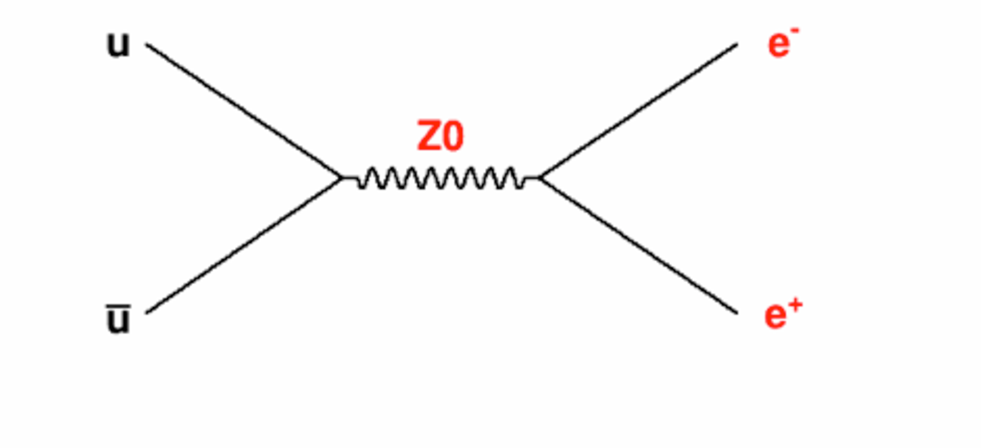
\includegraphics[scale=0.5]{./ElementaryParticles/Pictures/fig8.pdf}
\caption{LO Feynmann diagram for production of an electron position pair via a Z boson through the annihilation of an up and anti-up}
\label{fig:fig8}
\end{figure}
 

Figure ~\ref{fig:fig9} shows a NNLO (in the strong force) diagram for the same process.
 
\begin{figure}[h]
\centering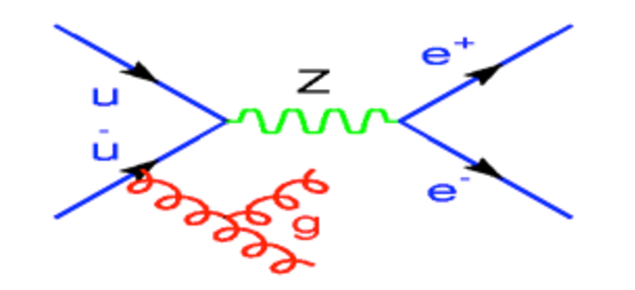
\includegraphics[scale=0.5]{./ElementaryParticles/Pictures/fig9.pdf}
\caption{NLO Feynmann diagram for production of an electron position pair via a Z boson through the annihilation of an up and anti-up}
\label{fig:fig9}
\end{figure}


\section{Non-Fundamental (composite) particles}
Apart from fundamental particles, more than 200 subatomic particles (made up of known fundamental particles) have been discovered using particle accelerators and detectors (see http://pdg.lbl.gov for a listing of the known particles).  These composite particles are made up of quarks, and are of two types:
\begin{itemize}
\item {\bf Baryons} are made of three quarks, for example neutron and proton.
\item {\bf Mesons} are made of quark pairs for example pions.
\end{itemize}
Baryons and mesons are collectively called Hadrons.




Mesons are bound states of 2 quarks.  These are very important for particle physics because, although the proton is the lightest stable particle, mesons are the lightest states containing quarks.  They are “unstable” -  meaning that they decay, sometimes very quickly, to other types of particles.
The lightest mesons are called pions.  There are three of them: one with a positive charge, one neutral, and one with a negative charge.  The charged pions decay via the weak force to a muon and a neutrino.  The neutral pion usually decays to two photons.
The naming conventions for all the mesons are very strange because the standard model and the existence of quarks was not yet understood when they were discovered.  Thus, there are “kaons” that contain strange quarks,and  “D mesons” that contain charm quarks.

As with hydrogen atoms, there are also excited states of the two bound quarks.  While with hydrogen, we just say “excited hydrogen”, with the mesons, the excited states often have separate names, as it was not understood at the time of their discovery that they were essentially “excited pions”.  Thus, rho mesons, eta mesons, etc are in a sense excited states of bound states of the up and down quark.

\section{The Higgs}
The  Higgs  boson  plays  a  special  role  in  the  standard  model.    Gauge
- invariant  quantum  field  theories generally 
predict  that  the  force  bosons  should  be  massless. And  indeed  the  photon  (E\&M),  the  gluon 
(strong force) are massless.  Although gravity can not yet be described by quantum field theory, in general a 
$1/r^2$ force indicates a massless boson, and gravity does
seem to follow this prescription.   Thus, naively, the 
standard model predicts that the W and Z boson should be massless.  However, instead, they have a mass 
about 100x that of the proton!  
The resolution was the Higgs.

The Higgs has several strange properties.  For all other particles, the lowest energy state is the one where there are no particles.  However, for the Higgs, the lowest energy state has a ``field'' of Higgs filling the universe.  The Higgs boson ``couples'' to the different fermions and the W and Z boson with different strengths (``coupling strengths'').  The stronger the coupling, the larger the mass of the particle, as the interactions with this Higgs field that fills the universe is larger.

The Higgs is the only particle in the standard model with a spin of zero (sometimes called a ``scalar'' particle).

\section{Further reading}
\begin{itemize}
\item pdg.lbl.gov is always a great site for all things related to particle physics
\item ``Modern Particle Physics'' by Mark Thomson
\item ``Introduction to Elementary Particle Physics'' by Alessandro Bettini
\item ``Particle Physics: A Very Short Introduction'' by Frank Close
\item ``Introduction to Elementary Particles'' by David Griffiths
\end{itemize}


